
\section{Introduction}

One of the main aspects of a biological community is its food web.
The first models of population dynamics generally considered the interactions between only
two species (e.g., \citet{canale1970}; \citet{rosenzweig1963}). However, in nature, food webs wherein
two species only influence the behaviour of the network are quite uncommon -- most
networks are far more complex \citep{hastings1991}. Therefore, several researchers asserted
that every food web study should involve at least three species in order to capture that
complexity \citep{price1980, rosenzweig1973}.

At first, the principal interest of food web researchers was in equilibrium analysis
because they assumed that what was observed in nature represented an equilibrium state.
Afterwards, different studies declared that chaos played an important role in ecological
models. The simplest definition of chaos is the extreme sensitivity of a system to its
initial conditions \citep{hastings1993}. This concept has been incorporated in population
dynamics since the mid-1970's.
Since then, many papers reinforced the importance of chaos in ecology.

\citet{hastings1991}, who studied chaos in a continuous time model of a food web including three
species, contributed considerably to the significance and understanding of this subject.
Their pioneering study led to many other papers on food webs dynamics and chaos
\citep{brose2006, gakkhar2012}. Replicating this kind of paper is important for many reasons.
For example, we can compare our results, obtained using current technologies, with theirs;
we can also make available the code written to recreate the model.
In the current paper, we used the same equations and parameters values as \citet{hastings1991} to replicate their model.
We were able to reproduce all the figures in their paper using \textit{Julia v1.3.1}.

\section{Methods}

The model formulation used in this paper is the same as the one in the original
publication. \citeauthor{hastings1991} used a 14 parameter model to represent the three-species
food chain, with $X$, $Y$, and $Z$ as the numbers of the species at the lowest level of
the food chain, of the species that preys upon $X$, and of the species that preys upon
$Y$, respectively.
However, all of their analyses are based on a simpler version of the model with
nondimensional measures of time and population sizes, hence 10 parameters only, with $x$,
$y$ and $z$ as the standardized abundances of the three species.
We chose to present this simpler nondimensional version only in this paper, and we invite
readers to consult \citeauthor{hastings1991}'s paper for more details on the original dimensional
parameters. Our model's formulation is given as:

\begin{equation} \label{eq:1}
  \begin{align}
    dx/dt &= x(1 - x) - f_1(x)y \\
    dy/dt &= f_1(x)y - f_2(y)z - d_1y \\
    dz/dt &= f_2(y)z - d_2z
  \end{align}
\end{equation}

with

\begin{equation} \label{eq:2}
    f_i(u) = a_iu/(1 + b_iu)
\end{equation}

as the functional response.

The parameter values used in this paper are the same as the ones in the original paper
(\autoref{tbl:table1}). However, the initial conditions of the simulations (i.e. the values of $x$,
$y$ and $z$ at the start) were not given in the original paper.
This is an important point, as the initial conditions strongly affect the simulations,
particularly in the context of chaotic behaviour.
We knew from Fig.3 of the original paper that $x \approx 0.76$.
We tried to approximate $y$ and $z$ by trial and error, and found $x = 0.76$, $y = 0.16$ and
$z = 9.9$ to be an appropriate combination for most cases.
We adapted the initial conditions in some simulations to give the closest matching
graphical result to the original figures.
The conditions used are specified in each figure caption.
We consider this a successful replication, despite the impossibility of using precisely
the same initial conditions.

\begin{table}[!htb]
  \centering
  \caption{Nondimensional parameters and the values used in the simulations}
  \label{tbl:table1}
  \begin{tabular}{c l}
    \hline
    Nondimensional parameters & Values \\
    \hline
    $a_1$ & 5.0 \\
    $b_1$ & 2.0 $\rightarrow$ 6.2 \\
    $a_2$ & 0.1 \\
    $b_2$ & 2.0 \\
    $d_1$ & 0.4 \\
    $d_2$ & 0.01 \\
    \hline
  \end{tabular}
\end{table}

As noted by \citeauthor{hastings1991}, numerical integration is the only way to investigate the
global dynamical behaviour of the system.
We used \textit{Julia v1.3.1} \citep{bezanson2017}, along with packages \verb| DifferentialEquations.jl|
\citep{rackauckas2017} to compute the numerical integrations and \verb|ParameterizedFunctions.jl|
\citep{rackauckas2017} to simplify the parameterized function call, as well as \verb|Plots.jl| to represent
our results. We let the \verb|solve()| function select the appropriate algorithm to solve our
differential equations.
In our implementation, it selected a composite algorithm combining, amongst others,
algorithms Tsit5 and Rosenbrock23.

To fully replicate the key findings of the original paper, we focussed on replicating the
original figures.
Here we describe the steps we took for Fig. 2, 3, 4 and 5 from the original paper.

Fig. 2 illustrated the chaotic behaviour of the system in time for each species.
In order to replicate it, we followed \citeauthor{hastings1991}'s method and let our system run
for 10 000 time steps.
We then represented the system's behaviour by plotting the species nondimensional
variables against time (between time steps 5000 and 6500, which eliminates transient
behaviour), as well as a three dimensional phase plot of the three species (for all time
steps). Note that in the case of the three dimensional phase plot, we had to set RK4 as
the solving algorithm, as well as a relative tolerance of $1e-14$; otherwise, the
representation was unexpectedly different from the original paper.
In order to illustrate the dynamics of the model, we created a Graphics Interchange Format
(GIF) file of the three-dimensional phase plot that showed the trajectories of $x$, $y$
and $z$ for the selected parameters (in supplement of this paper).

Fig. 3 showed the divergence of trajectories caused by a small change in initial
conditions when the system exhibited chaotic behaviour.
To replicate the figure, we plotted the trajectory for species $x$ between time steps 0
and 500 starting at $x = 0.77$, then changed the initial $x$ value by 0.01 (to $x = 0.78$)
and plotted the new trajectory for the same interval on the same graph.

Fig. 4 illustrated the appearance of chaotic behaviour as a function of changes in
$b_1$. To replicate it, we constructed a bifurcation diagram for species $z$ where we
varied values of $b_1$ from 2.2 to 6.2 in steps of 0.01. However, our approach had to be
slightly different.
\citeauthor{hastings1991} constructed what we consider a special type of bifurcation diagram,
representing only the maxima of $z$ as a function of $b_1$, rather than all possible
values in the system's behaviour, as in a typical logistic bifurcation diagram.
This raised the problem of correctly identifying the maximum values in the cycling
dynamic. Moreover, \citeauthor{hastings1991} mentioned that, in order to clarify their figure,
they eliminated points resulting from the secondary local maxima in the cycling dynamics
of species $z$, but they did not provide details on how they identified such points.
Hence, we adopted the following method:
1) we selected the 1000 last solutions for our system between time steps 1 and 10 000, in
order to eliminate transient behaviour;
2) we selected the values that were greater than both their preceding and following
values, which identified local maxima only;
and 3) we only kept values that were greater than a given threshold of the cycle's maximal
amplitude, in order to remove secondary local maxima.
We determined by trial and errors that the best threshold was 66\%, as it best removed
values in apparent second branches of $b_1$ while keeping the values in the primary
branch. We note however that for some values of $b_1$, the true solutions of the system
were unstable and that the system did not reach a cycling behaviour within 10 000 steps.
For these values of $b_1$ (37 values, all between 5.01 and 6.2), we could not present any
values of $z$ in our bifurcation diagram.

\citeauthor{hastings1991} mentioned in their original paper that they also examined the system's
behaviour when varying $b_2$ instead of $b_1$, although they did not present the results.
We examined the same behaviour by constructing another bifurcation diagram of $z$ for
values of $b_2$ varying from 1.5 to 3.2, using the same method as described above.
We fixed $b_1 = 3.0$, as it is the example used to illustrate chaotic behaviour throughout
\citeauthor{hastings1991}'s paper.

Fig. 5 illustrated another diagnostic feature of chaos, slopes of high magnitude on a
Poincaré map, for values of $b_1$ where the bifurcation diagram suggested chaotic
behaviour. In order to replicate this figure, we solved the system of differential
equations using the abovementioned algorithm RK4, as well as a relative tolerance of
$1e-14$. We used $b_1 = 3.0$ and $b_1 = 6.0$, as in the original paper, to replicate its
subfigures A-B and C-D, respectively.
We defined planes of equation $z = 9.0$ and $z = 3.0$ for those subfigures, respectively,
as these intercepted the "handles" of their respective three-dimensional phase plot.
We defined those "handles" as in \citeauthor{hastings1991}, that is as the region in the phase
plots where z declines from its maxima to its minima.
However, we had to use a tolerance value $epsilon$ of 0.05 in order to identify the points
whose distance from the plane was negligible (i.e. their $z$ values ranging between
8.95-9.05 and 2.95-3.05, respectively), since we were not able to find the phase plots'
exact interception points.
We specified the planes' $x$ and $y$ coordinates to retain only the points that were in
the "handles" (subfigures A,B: $x$ and $y$ ranging between 0.95-0.98 and 0.015-0.040,
respectively; subfigures C,D: $x$ and $y$ ranging between 0.93-1.00 and 0.00-0.09,
respectively).
As in the original paper, we recreated the Poincaré sections (subfigures A,C), by
plotting $y$ against $x$ coordinates of the retained points, and the Poincaré maps
(subfigures B,D), by plotting $x$ coordinates of the retained points $x(n)$
against that of their immediate subsequent retained points $x(n+1)$. Since Hastings and
Powell's Fig. 5E only schematized the plane in the three-dimensional phase plot, we
did not reproduce it.

The objective of this paper being to reproduce the main results of the original paper, we
did not reproduce its Fig. 1, which was only a schematic representation of the
three-species food chain.
All the code used to replicate the original paper is available alongside the article.

\section{Results}

We were able to replicate \citeauthor{hastings1991}'s main findings, even without knowing their
exact algorithm and initial values.
First, our time series of the nondimensional variables (\autoref{fig:fig2}) presents similar
qualitative results as those identified by \citeauthor{hastings1991}.
We observed that the standardized population densities of $x$, $y$, and $z$ (\autoref{eq:1}, \autoref{eq:2})
oscillate with a period of around 125 time steps.
Within a cycle, the population densities of species $x$ and $y$ oscillate while that of
species $z$ grows until it reaches its primary local maximum (see definition in methods),
at which $y$ and $x$ respectively reach their local minimum and maximum values.
$z$ then declines until it reaches its local minimum, forming the "handle" of the teacup
(\autoref{fig:fig2d}), and subsequently beginning a new cycle.
The animated figure we produced illustrates this dynamic (see supp.
online material).
Although slight discrepancies exist between our results and those of \citeauthor{hastings1991},
they did not seem to strongly influence the abovementioned period length, nor the values
of the local maxima and minima of the dimensionless variables.
Indeed, $x$ varies approximately from 0.2 to 1.0, $y$ from 0.0 to 0.4, and $z$ from 7.5 to
10.5 (\autoref{fig:fig2}), as seen in the original paper.

Second, the time series of $x$ from $t = 0$ to $500$ supports the chaotic behaviour of the
system, with slightly different initial conditions leading to increasingly different
trajectories(\autoref{fig:fig3}). The values themselves are almost identical to \citeauthor{hastings1991}'s
until $t \approx 250$, at which point they start to diverge, but this behaviour was to be
expected without the exact same initial conditions.

Third, our bifurcation diagrams (\autoref{fig:fig4}) have the same general shapes as the ones of
\citeauthor{hastings1991}, and are in the same range of $z_{max}$. We identified most of the
local maxima of $z$ found in the original paper for $b_1$ ranging from 2.2 to 6.2.
However, we missed some of them and we found others that were absent in their paper.
For instance, for $b_1$ = 3.1, we found multiple local maxima of $z$, whereas \citeauthor{hastings1991} had only found a dichotomy of values.
The differences are even more apparent in \autoref{fig:fig4}c, which represents a detailed
portion of \autoref{fig:fig4}a. For example, contrary to their findings, we did identify local
maxima values for $b_1$ ranging from 2.30 and 2.35. In other words, we did not observe the
significant gap in the bifurcation diagram that they had found.

Our additional bifurcation diagrams, where we varied $b_2$ instead of $b_1$ (\autoref{fig:figS1}),
confirm that chaos occurs for values other than $b_2$ = 2.0. Chaos is apparent for both
smaller or greater values.
However, while \citeauthor{hastings1991} reported that chaos was more likely for greater values of
$b_2$, our results highlight that $z$ instead converges to a single value and starts to
crash past $b_2$ = 2.35.

Lastly, although \citeauthor{hastings1991} did not specify the equation of the plane that
crosses the trajectories of the phase plot at its "handle", we were able to accurately
replicate their Poincaré section and map for $b_1$ = 3.0 (\autoref{fig:figS1} a,b). The main
discordance lies in the number of points that cross the plane, and consequently on the
apparent smoothness of the plots.
On the other hand, it was harder to precisely replicate the Poincaré map for $b_1$ = 6.0
(\autoref{fig:figS1}d), even though the corresponding reproduced Poincaré section (\autoref{fig:figS1}c)
was similar to the one in \citeauthor{hastings1991}'s paper.

\section{Discussion}

We were able to replicate the chaotic behaviour displayed by \citeauthor{hastings1991}'s model.
The resulting behaviour is indeed very sensible to the initial conditions, showing
increasingly diverging trajectories (\autoref{fig:fig3}) for slightly different parameters, as well
as unending oscillations (\autoref{fig:fig2}). The bifurcation diagrams (\autoref{fig:fig4}) further confirm
the existence of chaos by illustrating the presence of cyclic behaviour for some values
and chaotic intervals for others, hence the extreme sensibility of the system to $b_1$
values. As for the Poincaré sections (\autoref{fig:figS1} a,c), \citeauthor{hastings1991} plotted (x,y)
coordinates of points of the phase plots that theoretically coincided with the plane in
the "handle" of the teacup-shaped diagrams.
The Poincaré sections being almost unidimensional, we considered, as explained in the
original paper, a single variable within our Poincaré maps (\autoref{fig:figS1} b,d). The slopes
of these latter graphs therefore also denoted chaos, as specified by \citeauthor{hastings1991}.

For \autoref{fig:fig2} and \autoref{fig:fig3}, the shape of the cycles and oscillations are similar to
\citeauthor{hastings1991}'s.
As mentioned earlier, the slight differences are due to the fact that we could not use the
exact same initial conditions as the original authors.
Such difference is to be expected with a system exhibiting chaotic behaviour and do not
alter the conclusions.

The difference between our \autoref{fig:fig4} and \citeauthor{hastings1991}'s bifurcation diagram is more
intriguing. Admittedly, we could not figure out exactly what \citeauthor{hastings1991}'s method
was, and some elements such as identifying maxima values by increasing $b_1$ first, then
by decreasing it, did not make sense to us.
Our method should be appropriate, theoretically, to select only values that are primary
local maxima, and it did seem to work very well for most $b_2$ values;
yet, the broad range of values that we observed at $b_1$ = 3.1 instead of a dichotomy is
hard to explain.
It seems unlikely that the problem could be related to our arbitrary threshold of 66\% or
to our identification of a local maximum, because we would then either miss some lower
values or have too many, not having more in between.
The timeseries of all values of $z$ (not presented here) for $b_1$ = 3.1 confirms that
there are "intermediate" maxima values, which should be selected by any proper method.
We suggest that the difference might be due to the algorithms used for the numerical
integration in our two studies.
It is possible that the relationship between the parameters at this point is such that a
small difference in algorithm might have an important impact.
It is also possible that their algorithm came up with an unstable solution and a system
that did not reach cycling behaviour, such as ours for certain values past $b_1$ = 5.01,
but that \citeauthor{hastings1991}'s method selected some values anyways, explaining the behaviour
at $b_1$ = 3.1.

While we also found chaos for values of $b_2$ other than the default one of 2.0, both
smaller or greater, we do not totally agree with \citeauthor{hastings1991} that "chaos is more
likely for larger values of $b_2$". As \autoref{fig:figS1}, chaos can be quite likely for both
smaller or larger values.
We find important to note, however, that at a certain value of $b_2$, $z$ converges and
starts to crash, thus exhibiting non chaotic behaviour within a given range of $b_1$
values. This crash is to be expected when looking at the original dimensional parameters,
so it is possible that \citeauthor{hastings1991} simply chose not to reach this limit in their
analyses, as they were only interested in biologically reasonable parameters likely to
occur with the three species present.

We believe that our mixed results in attempting to replicate \autoref{fig:figS1} came from the
algorithm we used to identify the points that coincided with the plane.
For instance, we had to specify a tolerance value ($epsilon$), which defined a region
under and above the plane.
Although we were able to precisely replicate the Poincaré sections for $b_1$ = 3.0
(\autoref{fig:figS1}a) and 6.0 (\autoref{fig:figS1}c), the Poincaré maps need some refinement.
For $b_1$ = 3.0 (\autoref{fig:figS1}b), it lacked some points of the phase plots and included
others that were closed yet non-coincident with the plane.
For $b_1$ = 6.0 (\autoref{fig:figS1}d), the discrepancy was more obvious, and might be due to the
more chaotic behaviour of the system under this parameter, observed for example from the
larger width of its "handle" (compare axis intervals of \autoref{fig:figS1} a,c).

We have succeeded in replicating \citeauthor{hastings1991}'s model and its main findings, as our
results confirm chaos arising in a three species food chain in continuous time.
In general, the model, including its equations and parameters, was well described by the
authors. The most significant obstacles to reproducibility in \citeauthor{hastings1991}'s paper
were the absence of the values of the initial conditions, which have a huge impact on a
chaotic system, and the insufficient description of certain methods.
Consequently, there are slight differences between our results and theirs.
Furthermore, since we tried to keep our implementation as close as possible to the
original one, some steps did rely on arbitrary thresholds (for instance for the primary
local maxima or the boundaries of the Poincaré sections and maps).
Hence, our replication is somewhat not very flexible and possibly could not be applied to
a broader range of parameter values.
We suggest that an interesting step forward would be to train machine-learning algorithms,
such as neural networks, to identify chaotic behaviour and its boundaries, in order to
obtain an even better performing implementation.

\section{Author Contributions}
GD, FB and EB performed the first version of the reproduction and wrote the first version of the manuscript. AMD and TP provided guidance and comments during the reproduction, and revised the manuscript. GD performed the final revisions.

\section{Acknowledgments}
This reproduction was realized as part of the \textit{BIO6032 Biologie computationnelle et modélisation} course at Université de Montréal.

\newpage

\begin{figure}
  \centering
  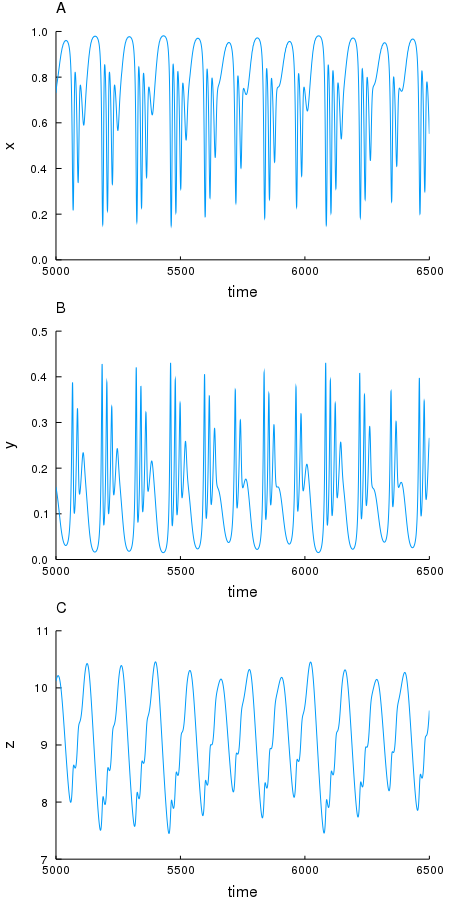
\includegraphics[scale=0.7]{figures/fig2.png} \caption{Time series of the nondimensional variables (a) $x$, (b) $y$ and (c) $z$, for $t$ ranging from 5000 to 6500 ($x$ = 0.76, $y$ = 0.16, and $z$ = 9.9 as initial conditions). The parameter values used in the simulations are given in \autoref{tbl:table1} ($b_1$ = 3.0). This figure replicates Fig. 2 A,B,C of \citet{hastings1991}.}
  \label{fig:fig2}
\end{figure}

\newpage

\begin{figure}
  \centering
  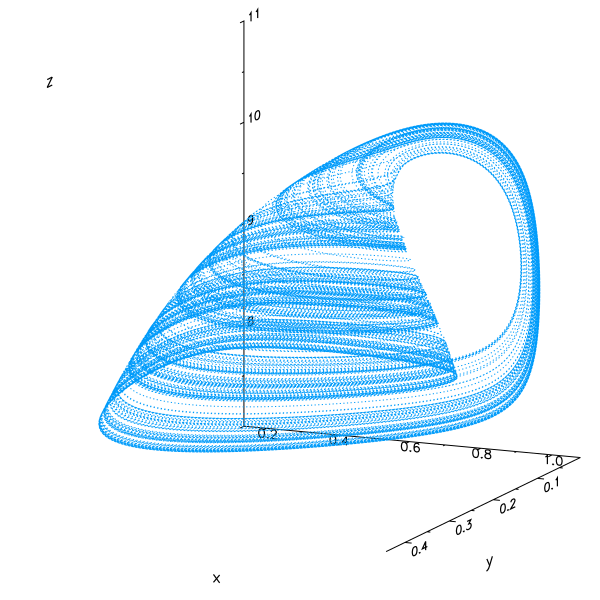
\includegraphics[scale=0.7]{figures/fig2d.png}
  \caption{Three-dimensional phase plot of species $x$, $y$ and $z$ for $t$ ranging from 1 to 10 000 ($x$ = 0.76, $y$ = 0.16, and $z$ = 9.9 as initial conditions). The parameter values used in the simulations are given in \autoref{tbl:table1} ($b_1$ = 3.0). This figure replicates Fig. 2D of \citet{hastings1991}.}
  \label{fig:fig2d}
\end{figure}

\newpage

\begin{figure}
  \centering
  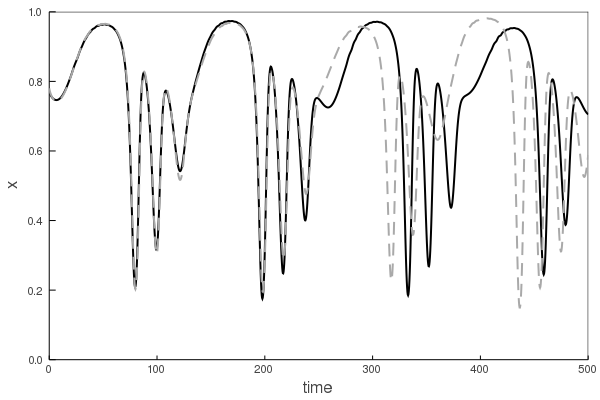
\includegraphics[scale=0.7]{figures/fig3.png}
  \caption{Time series of $x$, for $t$ ranging from 0 to 500. The solid and dashed lines have  $x$ = 0.77 and $x$ = 0.78 as initial conditions respectively ($y$ = 0.16 and $z$ = 9.9 as initial conditions are unchanged). The parameter values used in the simulations are given in \autoref{tbl:table1} ($b_1$ = 3.0). This figure replicates Fig. 3 of \citet{hastings1991}.}
  \label{fig:fig3}
\end{figure}

\newpage

\begin{figure}
  \centering
  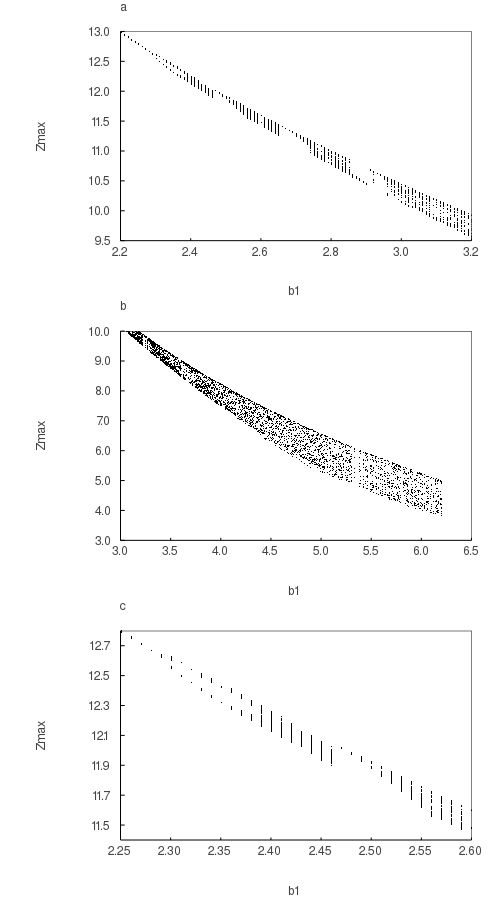
\includegraphics[scale=0.7]{figures/fig4.png}
  \caption{Bifurcation diagrams of the local maxima of $z$ plotted against $b_1$ ranging from (a) 2.2 to 3.2, (b) 3.0 to 6.2, and (c) 2.25 to 2.6. The other parameter values used in the simulations are given in \autoref{tbl:table1} ($x$ = 0.76, $y$ = 0.16, and $z$ = 9.9 as initial conditions). This figure replicates Fig. 4 of \citet{hastings1991}.}
  \label{fig:fig4}
\end{figure}

\newpage

\begin{figure}
  \centering
  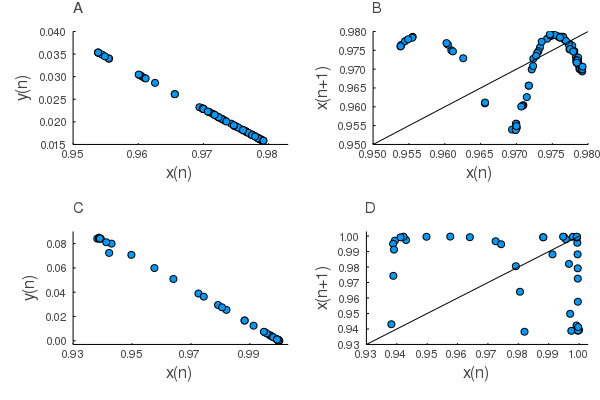
\includegraphics[scale=0.7]{figures/fig5.png}
  \caption{(a) and (b) Poincaré section and map, respectively, for the parameter values given in \autoref{tbl:table1} ($b_1$ = 3.0).  (c) and (d) Poincaré section and map for the same parameter values except $b_1$ = 6.0. All sets of initial values are unchanged ($x$ = 0.76, $y$ = 0.16, $z$ = 9.9). The solid lines of equation $x(n+1) = x(n)$ are shown in (b) and (d). This figure replicates Fig. 5 of \citet{hastings1991}, except their Fig. 5E, which is partly reproduced in \autoref{fig:fig2d}.}
  \label{fig:fig5}
\end{figure}

\newpage

\begin{figure}
  \centering
  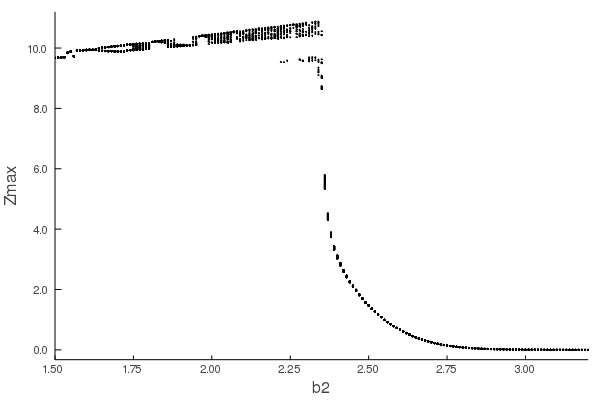
\includegraphics[scale=0.7]{figures/figS1.png}
  \caption{Bifurcation diagrams of the local maxima of $z$ plotted against $b_2$ ranging from 1.5 to 3.2. The other parameter values used in the simulations are given in \autoref{tbl:table1} ($x$ = 1.0, $y$ = 1.0, and $z$ = 1.0 as initial conditions, $b_1$ = 3.0).}
  \label{fig:figS1}
\end{figure}
